\begin{figure}[h] 
\centering 
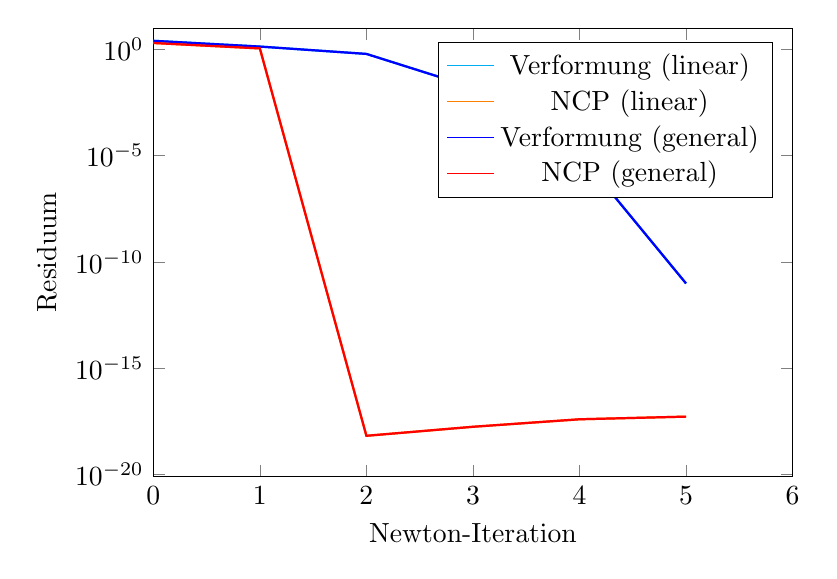
\begin{tikzpicture}[every plot/.append style={thick}] 
\begin{axis}[ 
label style={font=\normalsize}, 
xlabel={Newton-Iteration}, 
ylabel={Residuum}, 
xmin=0, xmax=6, 
ymode=log, 
ymin=0, ymax=10, 
width=0.8\textwidth, 
height=0.6\textwidth, 
legend pos=north east, 
legend style={cells={align=left}}, 
grid style=dashed, 
] 
\addplot[ 
color=cyan, 
] 
coordinates { 
(0, 2.56e+00)(1, 1.37e+00)(2, 6.18e-01)(3, 1.61e-02)(4, 1.20e-05)(5, 9.66e-12)}; 
\addlegendentry{Verformung (linear)} 
\addplot[ 
color=orange, 
] 
coordinates { 
(0, 2.02e+00)(1, 1.12e+00)(2, 6.51e-19)(3, 1.73e-18)(4, 3.90e-18)(5, 5.20e-18)}; 
\addlegendentry{NCP (linear)} 
\addplot[ 
color=blue, 
] 
coordinates { 
(0, 2.56e+00)(1, 1.37e+00)(2, 6.18e-01)(3, 1.61e-02)(4, 1.20e-05)(5, 9.66e-12)}; 
\addlegendentry{Verformung (general)} 
\addplot[ 
color=red, 
] 
coordinates { 
(0, 2.02e+00)(1, 1.12e+00)(2, 6.51e-19)(3, 1.73e-18)(4, 3.90e-18)(5, 5.20e-18)}; 
\addlegendentry{NCP (general)} 
\end{axis} 
\end{tikzpicture} 
\caption{Residuen des Stoffgesetzes 'St.Venant' mit Hinderniss 'Hut' und 50 Freiheitsgraden für die Verschiebung.} 
\label{fiq:St.Venant_Hut_level1} 
\end{figure} 
